
\section{Reproducibility}
\label{sec:reproducibility}

\subsection{Standardized task descriptions}

\begin{marginfigure}[1.75cm]
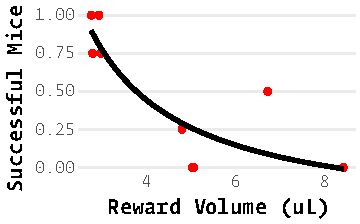
\includegraphics[]{figures/calibration_warning.pdf}
\caption{\textbf{"Minor" details have major effects.} Proportion of mice (each point, n=4) that were successful learning the first stage of the speech task described in \citep{saundersMiceCanLearn2019} across 10 behavior boxes with variable reward sizes. A $2 \mu L$ difference in reward size had a surprisingly large effect on success rate.}
\label{fig:calibration}
\end{marginfigure}

The implementation and fine details of a behavioral experiment matter. Seemingly trivial details like milliseconds of delay between trial phases and microliters of reward volume can be the difference between a successful and unsuccessful task (Figure \ref{fig:calibration}). \textit{Reporting} those details can thus be the difference between a reproducible and unreproducible result.  Researchers also often use "auxiliary" logic in tasks---such as methods for correcting response bias---that are never completely neutral to the interpretation of results. These too can be easily omitted due to brevity or memory in plain-English descriptions of a task, such as those found in Methods sections. Even if all details of an experiment were faithfully reported, the balkanization of behavioral software into systems peculiar to each lab (or even to individuals within a lab) makes actually performing a replication of a behavior result expensive and technically challenging. Widespread use of experimental tools that are not explicitly designed to preserve every detail of their operation presents a formidable barrier to rigorous and reproducible science\citep{wallReliabilityStartsExperimental2019}.

%
\begin{marginfigure}[1.1cm]
\begin{minted}[frame=lines,fontsize=\small]{json}
{
"step_name"    : "tone_discrim",
"task_type"    : "2AFC",
"bias_mode"    : 0,
"punish_sound" : false,
"stim" : {
  "sounds" : {
    "L": {
      "duration"  : 100,
      "frequency" : 10000,
      "type"      : "tone",
      "amplitude" : 0.01},
    "R": {"...":"..."}}},
"reward": {
  "type"     : "volume",
  "volume"   : 20},
"graduation" : {
    "type"      : "accuracy",
    "threshold" : 0.75,
    "window"    : 400},
}
\end{minted}
\caption{Task parameters are stored as portable JSON, formatting has been abbreviated for clarity.}
\label{fig:params}
\end{marginfigure}%
%
%
Autopilot splits experiments into a) the \textbf{code} that runs the experiment, which is intended to be standardized and shared across implementations, and b) the \textbf{parameters} (Figure \ref{fig:params}) that define your particular experiment. For example, two-alternative forced choice tasks have a shared structure regardless of the stimulus modality, but only your task plays pitch-shifted national anthems. Critically, this division of labor enables the possibility of developing a shared library of tasks as described in \hyperref[sec:expansion]{section \ref{sec:expansion}}%

The practice of reporting exactly the parameter description used by the software to run the experiment removes any chance for incompleteness in reporting. Because all task parameters are included in the produced data files, tasks are fully portable and can be reimplemented exactly by anyone that has comparable hardware to yours. 

\subsection{Self-Documenting Data}
\label{sec:data}

A major goal of the open science movement is to normalize publishing well-documented and clearly-formatted data alongside every paper. Typically, data are acquired and stored in formats that are lab-idiosyncratic or ad-hoc. Making data publishable then requires a laborious cleaning process. In the worst-case scenario, this cleaning process unearths some critically missing information about the experiment, requiring awkward caveats in the Methods section. Moreover, without careful version control, any changes made to the task code or parameters can be lost, making it difficult to compare last week's data to last month's.

\begin{marginfigure}[0.5cm]
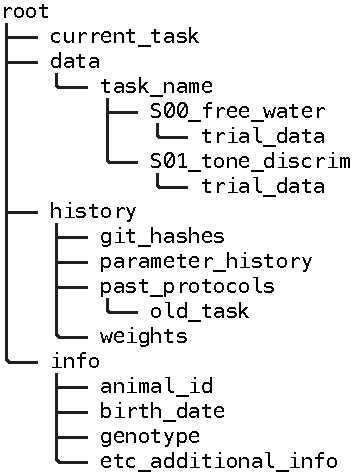
\includegraphics[]{figures/side_16_data.pdf}
\caption{Example data structure. All information necessary to reconstruct an experiment is automatically stored in a human-readable HDF5 file.}
\label{fig:datastx}
\end{marginfigure}

The best way to make data publishable is to avoid cleaning data altogether and \textit{design good data hygiene practices into the data acquisition process.} Autopilot automatically stores all the information required to fully reconstruct an experiment, including any changes in task parameters or code version that happen throughout training as the task is refined.

Autopilot data is stored in \href{https://support.hdfgroup.org/HDF5/whatishdf5.html}{HDF5} files, a hierarchical, high-performance file format. HDF5 files support metadata throughout the file hierarchy, allowing annotations to natively accompany data. Because HDF5 files can store nearly all commonly used data types, data from all collection modalities---trialwise behavioral data, continuous electrophysiological data, imaging data, etc.---can be stored together from the time of its acquisition. Data is always stored with the conditions of its collection, and is ready to analyze and publish immediately (Figure \ref{fig:datastx}). No Autopilot-specific scripts are needed to import data into your analysis tool of choice---anything that can read HDF5 files can read Autopilot data. 

In future versions we will implement the Neurodata Without Borders standard\citep{rubelNWBAccessibleData2019}, further enabling Autopilot data to be immediately incorporated into existing processing pipelines (see section \ref{sec:future}).

\subsection{Expense}
\label{sec:expense}

\begin{marginfigure}[2.6cm]
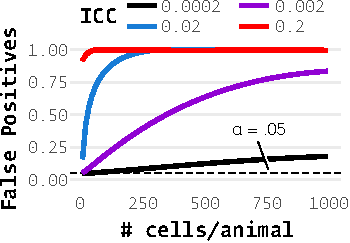
\includegraphics[]{figures/fpr.pdf}
\caption{When comparing a value across groups, eg. a genetic knockout vs. wildtype, even a modest intra-animal (or, more generally, intra-cluster) correlation (ICC) causes the false positive rate to be far above the nominal $\alpha = 0.05$. Shown are false positive rates for simulated data with various numbers of "cells" recorded for comparisons between two groups of 5 animals each with a real effect size of 0. We note that 741 simultaneously recorded cells were reported in \citep{junFullyIntegratedSilicon2017} and a mean ICC of 0.19 across 18 neuroscientific datasets was reported in \citep{aartsSolutionDependencyUsing2014}}
\label{fig:icc}
\end{marginfigure}

Autopilot is an order of magnitude less expensive than comparable behavioral systems (Table \ref{tab:cost}). We think the expense of a system is important for two reasons: scientific equity and statistical power. 

The distribution of scientific funding is highly skewed, with a large proportion of research funding concentrated in relatively few labs\citep{katzBiomedicalEliteInequality2017}. Lower research costs benefit all scientists, but lower instrumentation costs directly increase the accessibility of state-of-the-art experiments to labs with less funding. Since well-funded labs also tend to be concentrated at a few (well-funded) institutions, lower research costs also broaden the base of scientists outside traditional research institutions that can stay at the cutting edge\citep{ashkenasEvenAffirmativeAction2017,clausetSystematicInequalityHierarchy2015,pearceExpandingEquitableAccess2019}.



Neuroscience also stands to benefit from the lessons learned from the replication crisis in Psychology\citep{shroutPsychologyScienceKnowledge2018}. In neuroscience, underpowered experiments are the rule, rather than the exception\citep{buttonPowerFailureWhy2013}. Statistical power in neuroscience is arguably even worse than it appears, because large numbers of observations (eg. neural recordings) from a small number of animals are typically pooled, ignoring the nested structure of observations collected within individual animals. Increasing the number of cells recorded from a small number of animals dramatically increases the likelihood of Type I errors (Figure \ref{fig:icc})---indeed, for values of within-animal correlation typical of neuroscientific data, high numbers of observations make Type I errors more likely than not\citep{aartsSolutionDependencyUsing2014}. For this reason, perhaps paradoxically, recent technical advances in multiphoton imaging and silicon-probe recordings will actually make statistical rigor in neuroscience \textit{worse} if we don't use analyses that account for the multilevel structure of the data and correspondingly record from the increased number of animals that they require.




Although the expense of multi-photon imaging and high-density electrophysiology will always impose an experimental bottleneck, behavioral training time is often the greater determinant of study sample size. Typical behavioral experiments require daily training sessions often carried out over weeks and months, while far fewer imaging or electrophysiology sessions are carried out per animal.  Training large cohorts of animals in parallel is thus the necessary basis of a well-powered imaging or electrophysiology experiment.


\begin{table}
\caption{\textbf{Cost for Basic 2AFC System}\\
\noindent"Nosepoke" includes a solenoid valve, IR sensor, water tube, LED, housing, and any necessary driver PCBs.}
\label{tab:cost}
\noindent\begin{tabularx}{\linewidth}{XRRR}\toprule
& Autopilot & pyControl & Bpod  \\
\midrule
Behavior CPU & \href{https://www.adafruit.com/product/3775?src=raspberrypi}{\texttt{\$35}} & \href{http://www.open-ephys.org/store/pycontrol}{\texttt{\$284}} & \href{https://sanworks.io/shop/viewproduct?productID=1024}{\texttt{\$745}}\\
Nosepoke (3x) & \texttt{\$216} & \href{http://www.open-ephys.org/store/pycontrol-peripherals}{\texttt{\$579}} & \href{https://sanworks.io/shop/viewproduct?productID=1009}{\texttt{\$735}} \\
\textbf{Total for One} & \textbf{\texttt{\$251}} & \textbf{\texttt{\$920}} & \textbf{\texttt{\$1480}}\\
\midrule
Five Systems & \texttt{\$1255} & \texttt{\$4600} & \texttt{\$7400} \\
Host CPU(s) & \texttt{\$1000} & \texttt{\$5000} & \texttt{\$5000} \\
\textbf{Total for Five} & \textbf{\texttt{\$2255}} & \textbf{\texttt{\$9600}} & \textbf{\texttt{\$12400}} \\
\midrule
\textbf{Total for Ten} & \textbf{\texttt{\$3510}} & \textbf{\texttt{\$19200}} & \textbf{\texttt{\$24800}} \\
\bottomrule
\end{tabularx}
\end{table}
